\documentclass[12pt]{article}
\usepackage[margin=2.5cm]{geometry}
\usepackage{enumerate}
\usepackage{amsfonts}
\usepackage{amsmath}
\usepackage{fancyhdr}
\usepackage{amsmath}
\usepackage{amssymb}
\usepackage{amsthm}
\usepackage{mdframed}
\usepackage{graphicx}
\usepackage{subcaption}
\usepackage{adjustbox}
\usepackage{listings}
\usepackage{xcolor}
\usepackage{courier}
\usepackage[utf]{kotex}
\usepackage{hyperref}
\usepackage{soul}

\definecolor{codegreen}{rgb}{0,0.6,0}
\definecolor{codegray}{rgb}{0.5,0.5,0.5}
\definecolor{codepurple}{rgb}{0.58,0,0.82}
\definecolor{backcolour}{rgb}{0.95,0.95,0.92}

\lstdefinestyle{mystyle}{
    backgroundcolor=\color{backcolour},
    commentstyle=\color{codegreen},
    keywordstyle=\color{magenta},
    numberstyle=\tiny\color{codegray},
    stringstyle=\color{codepurple},
    basicstyle=\ttfamily\footnotesize,
    breakatwhitespace=false,
    breaklines=true,
    captionpos=b,
    keepspaces=true,
    numbers=left,
    numbersep=5pt,
    showspaces=false,
    showstringspaces=false,
    showtabs=false,
    tabsize=1
}

\lstset{style=mystyle}

\pagestyle{fancy}
\renewcommand{\headrulewidth}{0.4pt}
\lhead{CSC 369}
\rhead{Midterm 5 Solution}

\begin{document}
\title{CSC 369 Midterm 5 Solution}

\bigskip

\begin{enumerate}[1.]
    \item

    No. if the access is read for both threads, then concurrency error will not occur.

    \item

    \texttt{b)}, \texttt{c)} and \texttt{d)} are true

    \bigskip

    \begin{mdframed}
    \underline{\textbf{Correct solution}}

    \bigskip

    \texttt{c)} and \texttt{d)} are true
    \end{mdframed}

    \bigskip

    \underline{\textbf{Notes}}

    \begin{itemize}
        \item [\color{blue}Question\color{black}] What does it mean when mutex is held by this thread?
        \item [\color{blue}Question\color{black}] What I do know is that \texttt{pthread\_cond\_wait}
        puts thread to sleep. My question here is, how come the mutex is not held when thread is in a blocked state/sleep?
    \end{itemize}

    \item

    \begin{enumerate}[a)]
        \item

        Only \texttt{b)} causes starvation.

        \item

        Conditional variable is a queue that allows threads to be put themselves on to
        sleep (in blocked state) when thread it is not desired using \texttt{pthread\_cond\_wait}
        function.

        \bigskip

        Since there are no threads inside \texttt{cv1}, there is nothing to awake using
        \texttt{pthread\_cond\_signal}.

        \bigskip

        So, nothing will occur.

        \bigskip

        \item

        System call is a subset of interrupt caused by user application to switch
        from user mode to kernel mode to perform previleged operations for the application.

        \bigskip

        Interrupt is a signal sent by hardware (e.g keyboard, mouse, hard drive) or software.

        \bigskip

        It tells the cpu to stop its activities and execute appropriate part of the operating system.

        \bigskip

        \underline{\textbf{Notes}}

        \begin{itemize}
            \item I need to review how interrupt works. I had to look up the information.
            \item [\color{blue}Question\color{black}] How does interrupt work?
            \item \textbf{Interrupt}

            \begin{itemize}
                \item Is a signal
                \item there are two types of interrupts:
                \begin{itemize}
                    \item Hardware interrupt
                    \begin{itemize}
                        \item Is signal generated by hardware (e.g RAM is full, Hard drive is full)
                        \item Is sent to operating system
                    \end{itemize}
                    \item Software interrupt
                    \begin{itemize}
                        \item Is signal generated by software (e.g program crash, system call)
                        \item Is sent to operating system
                        \item May call trap instruction (esp. system call)
                    \end{itemize}
                \end{itemize}
            \end{itemize}

            \bigskip

            \begin{center}
            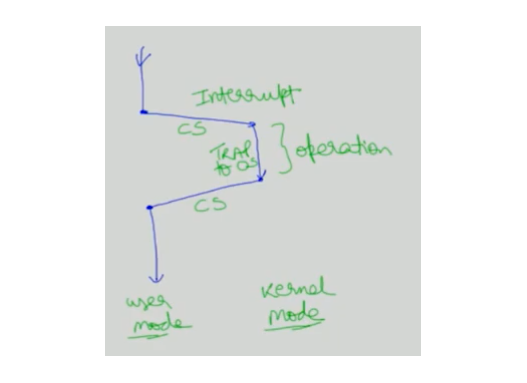
\includegraphics[width=0.8\linewidth]{../../images/midterm_5_solution_1.png}
            \end{center}
        \end{itemize}

        \bigskip

        \underline{\textbf{References}}

        \begin{enumerate}[1.]
            \item venkatesan ramachandran, What is an Interrupt?, \href{https://www.youtube.com/watch?v=NYTK65RrjnE&ab_channel=venkatesanramachandran}{link}
        \end{enumerate}

        \item

        No. This statment is false.

        \bigskip

        User level threads are generated in user-mode without kenerel being aware about it.

        \bigskip

        \bigskip

        \underline{\textbf{Notes}}

        \begin{itemize}
            \item [\color{blue}Question\color{black}] What is the difference between user-level thread
            and kernel-level thread?
            \item [\color{blue}Question\color{black}] Why is thread that is generated at user level using procedure
            call faster than kernel level thread?
            \item [\color{blue}Question\color{black}] What is procedure call? How does it work?

            \item \textbf{Procedure call}
            \begin{itemize}
                \item works in user-mode only
                \item doesn't require context switching
                \item doesn't need help from OS/Kernel
                \item no context-switching $\to$ faster
            \end{itemize}
        \end{itemize}

        \bigskip

        \underline{\textbf{References}}

        \begin{enumerate}[1.]
            \item Tech Dose, System call vs Procedure call, \href{https://www.youtube.com/watch?v=98uHzqmPABY&ab_channel=TECHDOSE}{link}
        \end{enumerate}

        \item

        System calls do not generate processes. \texttt{fork()} does.

        \bigskip

        With this reason the program \texttt{run\_stuff} generates only 1 additional process.

        \bigskip

        \underline{\textbf{Notes}}

        \begin{itemize}
            \item [\color{blue}Question\color{black}] What is a process? And how does process work?
            \item [\color{blue}Question\color{black}] How come system call doesn't generate process? And how come
            fork() generates process?

            \item \textbf{Process}

            \begin{itemize}
                \item Is a running program
                \item Has 3 states
                \begin{enumerate}[1.]
                    \item \textbf{Running:}
                    \begin{itemize}
                        \item means a processs is running on a processor
                        \item means instructions are being executed
                    \end{itemize}
                    \item \textbf{Ready:}
                    \begin{itemize}
                        \item means a process is ready to run
                        \item means OS has chosen not to run the program at the given moment
                    \end{itemize}
                    \item \textbf{Blocked:}
                    \begin{itemize}
                        \item means a process has performed some kind of operation that makes it not ready to run
                        until some event takes place
                    \end{itemize}
                \end{enumerate}
            \end{itemize}
        \end{itemize}
    \end{enumerate}

    \item

\begin{lstlisting}[language=c]
    typedef struct acct {
        float balance;
        pthread_mutex_t lock;
        pthread_cond_t cond;
    } account;

    void transfer_amount(account *a1, account *a2, float amount) {

        // lock critical section during the transfer process
        pthread_mutex_lock(&a1->lock);
        pthread_mutex_lock(&a2->lock);
        // transfer amount
        a1->balance -= amount;
        a2->balance += amount;
        pthread_mutex_lock(&a1->lock);
        pthread_mutex_lock(&a2->lock);

        // lock the transferring user if the balance is negative
        if (a1->balance < 0) {
            pthread_cond_wait(&a1->cond, &a1->lock);
        }

    }

\end{lstlisting}

    \bigskip

    \begin{mdframed}
    \underline{\textbf{Correct Solution}}

    \bigskip

\begin{lstlisting}[language=c]
    typedef struct acct {
        float balance;
        pthread_mutex_t lock;
        pthread_cond_t cond;
    } account;

    void transfer_amount(account *a1, account *a2, float amount) {

        pthread_mutex_lock(&a1->lock);
            a1->balance -= amount;

            while (a1->balance < 0) {
                pthread_cond_wait(&a1->cond, &a1->lock);
            }
        pthread_mutex_lock(&a1->lock);

        pthread_mutex_lock(&a2->lock);
            a2->balance += amount;

            if (a2->balance > 0) {
                pthread_cond_signal(&a2->cond);
            }
        pthread_mutex_lock(&a2->lock);
    }

\end{lstlisting}

    \end{mdframed}

    \bigskip

    \underline{\textbf{Notes}}

    \begin{itemize}
        \item Realized that I do not know how to create barriers to critical section.
        \item [\color{blue}Question\color{black}] When do we use the while loop like lock?
        \item [\color{blue}Question\color{black}] Does the use of if statement to put thread into sleep acceptable?
        \item [\color{blue}Question\color{black}] How can we construct safe barriers around critical section?
        \item \textbf{Locks}
        \begin{itemize}
            \item Ensures that any critical section executes is a signle atomic operation
            \item Guarentees that no more than single code can be active within the code
        \end{itemize}

        \item \texttt{pthread\_mutex\_lock}
        \begin{itemize}
            \item \textbf{Syntax:} \texttt{pthread\_mutex\_t VAR}
            \item Is used to provide mutual exclusion between threads
            \item If mutex is already locked, thread blocks until mutex is available
            \item Must be proerly initialized before use

            \bigskip

            \underline{\textbf{Static Way}}

            \bigskip

            \texttt{pthread\_mutex\_t lock = PTHREAD\_MUTEX\_INITIALIZER}

            \bigskip

            \underline{\textbf{Dynamic Way}}

            \bigskip

            \texttt{int rc = pthread\_mutex\_init(\&lock NULL);}\\
            \texttt{assert(rc == 0);}

            \bigskip

        \end{itemize}
    \end{itemize}

    \item

    \begin{enumerate}[a)]
        \item It would favour I/O bound process. I/O bound process are mostly about waiting for the completion
        of input or output.

        \bigskip

        And example of this is continuous typing on microsoft word.

        \bigskip

        Usually the I/O-bound process lasts a short period of time.

        \bigskip

        On the other hand, CPU-bound process involves the execution of algorithm that requires a
        huge computation time.

        \bigskip

        An example of this is running a simulation.

        \bigskip

        Because of this, CPU-bound process usually lasts a long period of time.

        \bigskip

        Because of this, the processing algorithm would favour I/O bound process
        over CPU bound process.

        \item

        Yes.

        \bigskip

        The processing algorithm favours algorithm with a short processing time in the past.

        \bigskip

        Using the explanation given in part a), we can write I/O bound processes are favoured
        over CPU-bound process

        \bigskip

        It follows from this information that if short I/O bound processes keep coming in,
        then CPU-bound process will never get a chance to run.

        \bigskip

        So, we can conclude the scheduling algorithm would cause starvation to CPU-bound processes.

    \end{enumerate}

    \item

    \begin{enumerate}[1)]
        \item

        \begin{enumerate}[a)]
            \item False
            \item True
            \item True
            \item False
            \item False
            \item False
        \end{enumerate}

        \item

        \begin{enumerate}[a)]
            \item Is one of simplest lock to build. It allows only one thread to enter at a time. The variable lock
            has two values 0 (free/available), 1 (in use/locked). Spinlock uses two operations. One is \texttt{acquire()}
            and another is \texttt{release()}. \texttt{acquire()} uses while loop and \texttt{test-and-lock} function to
            ensure atomic operation in critical section. A thread is in locked state until lock is freed.

            \item Is the amount of time where processes in the same queue runs until
            it repeats. The time slice or scheduling quantum must be a multiple of
            the time of timer-interrupt.

            \item Is a software interrupt sent by user application, so it
            traps into kernel mode, perform previliged operation, return to user mode from trap,
            and continue application with the returned result.
        \end{enumerate}

        \bigskip

        \underline{\textbf{Notes}}

        \begin{itemize}
            \item I feel weak about scheduling quantum
            \item [\color{blue}Question\color{black}] What is scheduling quantum?
        \end{itemize}
    \end{enumerate}

    \item

    \begin{enumerate}[1)]
        \item

        \begin{enumerate}[a)]
            \item True
            \item True
            \item False
            \item True
            \item False
            \item False
        \end{enumerate}

        \bigskip

        \begin{mdframed}
        \underline{\textbf{Correct Solution}}

        \bigskip

        \begin{enumerate}[a)]
            \item \color{red}False\color{black}
            \item True
            \item False
            \item True
            \item False
            \item False
        \end{enumerate}

        \end{mdframed}

        \bigskip

        \underline{\textbf{Notes}}

        \begin{itemize}
            \item I feel weak about PCB and context switch
            \item [\color{blue}Question\color{black}] What is response for changing from user mode to kernel mode on system call interrupt?
            \item [\color{blue}Question\color{black}] What is program counter?
            \item [\color{blue}Question\color{black}] What is stack pointer?
            \item [\color{blue}Question\color{black}] What is user register?
            \item [\color{blue}Question\color{black}] What is kernel state?
        \end{itemize}

        \item

        \begin{enumerate}[a)]
            \item Is a function that is a part of spin lock. It is used as a conditional statement in while
            loop to make sure only one thread can enter the critical at a time. Test and lock returns false
            if lock variable in spin lock is freed (with value of 0).

            \bigskip

            \begin{mdframed}
            \underline{\textbf{Correct Solution}}

            \bigskip

            Is an atomic instruction. It is used to implement syncrhonization algorithm such as spinlock.

            \end{mdframed}

            \bigskip

            \underline{\textbf{Notes}}

            \begin{itemize}
                \item I feel weak about test-and-set
            \end{itemize}

            \item

            Is a type of scheduling algorithm where one process is favoured and executed first
            over the others. Some examples are MLFQ and SJF scheduling algorithm.

            \bigskip

            \begin{mdframed}
            \underline{\textbf{Correct Solution}}

            \bigskip

            Is a type of scheduling algorhtm where a process can be interrupted by an OS. Once the
            time slice of a process is used, the next process is scheduled into running state.
            \end{mdframed}

            \bigskip

            \underline{\textbf{Notes}}

            \begin{itemize}
                \item I don't feel confident about preemtive scheduling and non-preemptive scheduling
                \item [\color{blue}Question\color{black}] What is preemptive scheduling?
            \end{itemize}
        \end{enumerate}
    \end{enumerate}

    \item

    \begin{enumerate}[a)]
        \item \texttt{c)} is the only scheduling algorithm that minimizes average wait time.
        \item

        \bigskip

        A conditional variable is a queue where an undesired thread can be added and put to sleep
        (by switching to blocked state) by calling the function \texttt{pthread\_cond\_wait}.

        \bigskip

        When state is changed, one or more threads in conditional variable can be awakend.

        \bigskip

        A thread in conditional variable is put to sleep using the function \texttt{pthread\_cond\_wait}

        \bigskip

        And a thread in conditional variable is awakend using the function \texttt{pthread\_cond\_signal}

        \bigskip

        Semaphore is a signal. It uses integer variable shared between multiple threads.

        \bigskip

        Semaphore has two types: counting semaphore and binary semaphore.

        \bigskip

        Counting semaphore has \texttt{count} variable where \texttt{count = 0} means
        resource is not avaiable.

        \bigskip

        Binary semaphore has \texttt{count} variable with two states \texttt{0 - locked / not available}
        \texttt{1 - available/free}.

        \bigskip

        A situation where a conditional variable is favored over the other variable
        is during banking transaction. Here, we use conditional variable to put a particular thread
        to sleep if condition is not satisfied (i.e balance remaining is negative).

        \bigskip

        \underline{\textbf{Notes}}

        \begin{itemize}
            \item I feel weak about conditional variable and semaphores
            \item [\color{blue}Question\color{black}] What is conditional variable?
            \item [\color{blue}Question\color{black}] What is semaphore?
            \item I feel that conditional variable is used to control specific thread
            where as semaphore is used to control a group of thread (like a traffic)
        \end{itemize}

        \item

        No.

        \bigskip

        Interrupt is a signal generated by either software or hardware.

        \bigskip

        It tells the cpu to stop its current activity and execute appropriate instruction
        int the operating system.

        \bigskip

        Mutual exclusion guarentees only one thread to enter critical section at a time.

        \bigskip

        The two are unrelated.

        \bigskip

        To achieve mutual exclusion, critical section must be atomic.

        \bigskip

        \texttt{pthread\_mutex\_lock()} is one of the locks that enforces mutual exclusion.

        \bigskip

        \underline{\textbf{Notes}}

        \begin{itemize}
            \item I feel weak about mutual exclusion
            \item [\color{blue}Question\color{black}] What is mutual exclusion?
            \item [\color{blue}Question\color{black}] What is necessary condition to ensure mutual exclusion?
        \end{itemize}

        \item

        I do not know but here is my best shot.

        \bigskip

        System call is a subset of interrupt sent by user application to context switch
        from user mode to kernel mode so previleged operations can be done.

        \bigskip

        User pointer is a pointer which points to an address in RAM dedicated for
        programs in user-mode.

        \bigskip

        When system call goes into kernel mode, it saves PC counter, CPU register, kernel state,
        and other resource information.

        \bigskip

        When a program returns from trap, it has to resume its program.

        \bigskip

        Before resuming program, we have to make sure all is well.

        \bigskip

        It is here where the validation of user pointer occurs.

        \bigskip

        \underline{\textbf{Notes}}

        \begin{itemize}
            \item [\color{blue}Question\color{black}] What is user pointer?
        \end{itemize}

        \item

        I do not know but here is my best shot

        \bigskip

        User-level thread is a thread generated in user-mode without OS knowing about it.

        \bigskip

        \underline{\textbf{Notes}}

        \begin{itemize}
            \item I feel week about user-level threads and kernel-level threads
            \item [\color{blue}Question\color{black}] What is user level thread?
            \item [\color{blue}Question\color{black}] What is kernel level thread?
        \end{itemize}

    \end{enumerate}

\end{enumerate}

\end{document}